% DOC SETTINGS ===================================
\documentclass{article}
\usepackage[utf8]{inputenc}
\usepackage{steinmetz}
\usepackage{mathtools}  
\usepackage{multicol}
\usepackage{circuitikz}
\usepackage{tikz}
\usepackage{listings}
\usepackage{geometry}
\usepackage{fancyhdr}
\usepackage{amsfonts}
\usepackage{media9}
\usepackage{parskip}
\usetikzlibrary{positioning, fit, calc}
\pagestyle{fancy}
\lhead{ECE2714 Problem Set 10}
\rhead{Kavin Thirukonda 2021}
\fancyheadoffset{0mm}
 \geometry{
 a4paper,
 total={170mm,257mm},
 left=20mm,
 top=25mm,
 }
\mathtoolsset{showonlyrefs} 
\cfoot{}
% DOC SETTINGS ===================================
\begin{document}
\begin{enumerate}
    \item Determine if the CT LTI system described by the LCCDE
    \begin{equation}
        \frac{d^3}{dt^3}y(t)-9\frac{d^2}{d^2}y(t) + 24\frac{d}{dt}y(t)+34y(t) = \frac{dx}{dt} +2x(t)
    \end{equation}
    is stable. Explain your rationale.
    \newpage
    \item Given a stable LTI system described by the LCCDE
    \begin{equation}
        \frac{d^3}{dt^3}y(t)+106\frac{d^2}{d^2}y(t) + 605\frac{d}{dt}y(t)+500y(t) = 100\frac{dx}{dt} +200x(t)
    \end{equation}
    \begin{enumerate}
        \item Find the frequency response of the system
        
        \item If the input to this system is x(t) = cos(t), what is the output in the time domain, y(t)?
    \end{enumerate}
    \newpage
    \item Given the Bode plot for a system as follows
    \begin{center}
        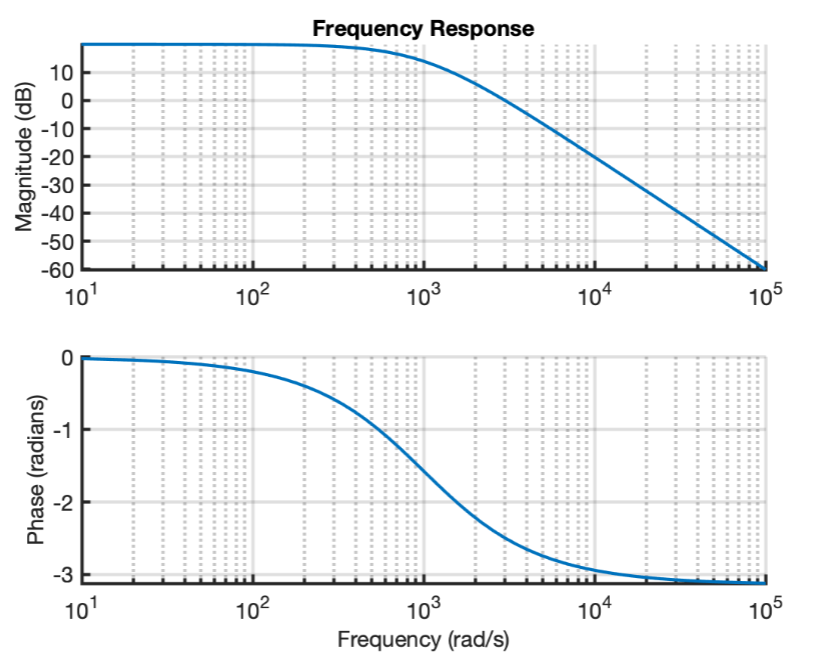
\includegraphics[width = .5\textwidth]{bode.png}
    \end{center}
    \begin{enumerate}
        \item What is the output if the input is $x(t) = e^{j100t}$?
        \item What is the output if the input is $x(t) = \sin(3000t)$?
        \item What is the output if the input is $x(t) = \cos(10000t - \frac{\pi}{100})$?
    \end{enumerate}
    \newpage
    \item The output y(t) of a causal LTI system is related to the input x(t) by the differential equation   
    \begin{equation}
        \frac{d}{dt}y(t) + 2y(t) = x(t).
    \end{equation}
    The input x(t) to the system is given as
    \begin{equation}
        x(t) = e^{-t}u(t).
    \end{equation}
    Determine the Fourier tranform of the output, $Y(j\omega)$.
    \newpage
    \item Consider the followign second-order  difference equation
    \begin{equation}
        y[n] + y[n-1] +\frac{1}{4}y[n-2] = x[n]
    \end{equation}
    Decide whether or not the step response is oscillatory and explain your reasoning.
    \newpage
    \item Consider a discrete time system that produces output
    \begin{equation}
        y[n] = n\left(\frac{4}{5}\right)^nu[n]
    \end{equation}
    when the input is
    \begin{equation}
        x[n] = \left(\frac{4}{5}\right)^nu[n]
    \end{equation}
    \begin{enumerate}
        \item Determine the system frequency response $H(e^{j\omega})$
        \item Determine the difference equation that defines the system
        \item Determine the system impulse response
    \end{enumerate}
\end{enumerate}
\end{document}
